% =====================================================================
%  EPIC 2026 — 5th Engineering Physics International Conference
%  FULL PAPER — AIP Conference Proceedings (AIPCP) format, 4–8 pages
%
%  Tenggat  : Full Paper 20 Sep 2026 | Revisi 15 Okt 2026 | Konferensi 24 Okt 2026
%  Kompilasi: latexmk -pdf main.tex            -> versi lengkap (main.pdf)
%             latexmk -pdf main_anon.tex       -> versi anonim (double-blind)
%
%  INTEGRITAS DATA: setiap angka hasil berasal dari generated/numbers.tex dan
%  generated/table_results.tex, dihasilkan oleh
%      swarm_ws/analysis/skema5_paper_analysis.py
%  dari 56 CSV + 8 log coordinator di
%      swarm_ws/src/swarm_sim/results/skema5_video_runs/  (lihat MANIFEST.json)
%  Jangan menulis angka hasil secara manual. Audit: generated/audit.md.
% =====================================================================
\documentclass[10pt,letterpaper]{article}

% ---------- Mode anonim (di-set oleh main_anon.tex) ----------
\providecommand{\anonymous}{0}
\newif\ifanon
\ifnum\anonymous=1 \anontrue \else \anonfalse \fi

% ---------- Halaman: margin AIP, TIDAK BOLEH diubah ----------
\usepackage[letterpaper,top=1in,bottom=1.18in,left=1in,right=1in]{geometry}

% ---------- Times New Roman untuk teks & matematika ----------
\usepackage[T1]{fontenc}
\usepackage[utf8]{inputenc}
\usepackage{amsmath,amssymb}
\usepackage{newtxtext,newtxmath}
\usepackage{setspace}
\singlespacing

\usepackage{graphicx}
\usepackage{booktabs}
\usepackage{array}
\usepackage{multirow}
\usepackage{caption}
\usepackage{changepage}
\usepackage{xcolor}
\usepackage{tikz}
\usetikzlibrary{arrows.meta,positioning,fit,backgrounds,calc,decorations.pathreplacing}
\usepackage{enumitem}
\usepackage[hidelinks]{hyperref}

\pagestyle{empty}

% ---------- Float ----------
\setcounter{topnumber}{3}
\setcounter{bottomnumber}{2}
\setcounter{totalnumber}{4}
\renewcommand{\topfraction}{0.92}
\renewcommand{\bottomfraction}{0.75}
\renewcommand{\textfraction}{0.07}
\renewcommand{\floatpagefraction}{0.75}
\setlength{\textfloatsep}{8pt plus 2pt minus 2pt}
\setlength{\floatsep}{6pt plus 2pt minus 2pt}

\setlength{\parindent}{0.2in}
\setlength{\parskip}{0pt}
\setlength{\abovedisplayskip}{4pt}
\setlength{\belowdisplayskip}{4pt}
\setlength{\abovedisplayshortskip}{2pt}
\setlength{\belowdisplayshortskip}{2pt}

% ---------- Caption AIP: 9 pt centered; FIGURE n. di bawah, TABLE n. di atas ----------
\DeclareCaptionLabelFormat{aipfigure}{\textbf{FIGURE #2.}}
\DeclareCaptionLabelFormat{aiptable}{\textbf{TABLE #2.}}
\captionsetup[figure]{labelformat=aipfigure,labelsep=space,font={small},
    justification=centering,singlelinecheck=true,skip=4pt}
\captionsetup[table]{labelformat=aiptable,labelsep=space,font={small},
    justification=centering,singlelinecheck=true,skip=3pt}

% ---------- Heading AIP ----------
\newif\ifafterheadone
\newcommand{\headingone}[1]{\par\addpenalty{-200}\vspace{8pt}%
    {\centering\fontsize{12}{14}\selectfont\bfseries\MakeUppercase{#1}\par}%
    \nopagebreak\vspace{3pt}\nopagebreak\global\afterheadonetrue\noindent\ignorespaces}
\newcommand{\headingtwo}[1]{\par\ifafterheadone\nopagebreak\else\addpenalty{-200}\fi\vspace{6pt}%
    {\centering\fontsize{12}{14}\selectfont\bfseries #1\par}%
    \nopagebreak\vspace{2pt}\nopagebreak\global\afterheadonefalse\noindent\ignorespaces}
\newcommand{\headingthree}[1]{\par\vspace{4pt}%
    {\centering\fontsize{10}{12}\selectfont\itshape #1\par}%
    \vspace{1pt}\noindent\ignorespaces}

% ---------- Bibliografi AIP (aipnum4-1 di kelas article) ----------
\usepackage[numbers,sort&compress]{natbib}
\providecommand{\bibinfo}[2]{#2}
\providecommand{\bibnamefont}[1]{#1}
\providecommand{\bibfnamefont}[1]{#1}
\providecommand{\citenamefont}[1]{#1}
\providecommand{\natexlab}[1]{#1}
\providecommand{\eprint}[2][]{\url{#2}}
\providecommand{\doibase}{https://doi.org/}
\providecommand{\urlprefix}{}
\providecommand{\Doi}[1]{\href{\doibase#1}{#1}}
\providecommand{\BibitemOpen}{}
\providecommand{\BibitemShut}[1]{}
\providecommand{\bibAnnote}[2]{}
\providecommand{\selectlanguage}[1]{}
\makeatletter
\renewcommand{\@biblabel}[1]{#1.}
\makeatother
\setlength{\bibsep}{0pt plus 0.5pt}

% ---------- Angka hasil (DIHASILKAN OTOMATIS) ----------
% DIHASILKAN OTOMATIS oleh swarm_ws/analysis/skema5_paper_analysis.py — JANGAN DIEDIT.
\newcommand{\CovRectHinf}{98.2}
\newcommand{\TmisRectHinf}{260}
\newcommand{\TninetysevenRectHinf}{240}
\newcommand{\LatrmsRectHinf}{7.2}
\newcommand{\LatpfiveRectHinf}{17.7}
\newcommand{\LatmedRectHinf}{3.0}
\newcommand{\VsweepRectHinf}{1.20}
\newcommand{\AltrmsRectHinf}{2.5}
\newcommand{\TiltpfiveRectHinf}{14.7}
\newcommand{\TiltmaxRectHinf}{21.1}
\newcommand{\EffortRectHinf}{0.054}
\newcommand{\SatRectHinf}{0.08}
\newcommand{\ObssurfRectHinf}{0.49}
\newcommand{\VtwovRectHinf}{1.71}
\newcommand{\DminlogRectHinf}{1.71}
\newcommand{\PtierRectHinf}{2.91}
\newcommand{\TiertwoRectHinf}{88}
\newcommand{\CovofflineRectHinf}{98.9}
\newcommand{\CovRectLqr}{n/a}
\newcommand{\TmisRectLqr}{78.8}
\newcommand{\TninetysevenRectLqr}{n/a}
\newcommand{\LatrmsRectLqr}{11.7}
\newcommand{\LatpfiveRectLqr}{23.4}
\newcommand{\LatmedRectLqr}{8.8}
\newcommand{\VsweepRectLqr}{1.12}
\newcommand{\AltrmsRectLqr}{7.3}
\newcommand{\TiltpfiveRectLqr}{14.7}
\newcommand{\TiltmaxRectLqr}{155.9}
\newcommand{\EffortRectLqr}{0.024}
\newcommand{\SatRectLqr}{0.11}
\newcommand{\ObssurfRectLqr}{0.06}
\newcommand{\VtwovRectLqr}{1.52}
\newcommand{\DminlogRectLqr}{1.52}
\newcommand{\PtierRectLqr}{n/a}
\newcommand{\TiertwoRectLqr}{n/a}
\newcommand{\CovofflineRectLqr}{42.6}
\newcommand{\CovLshapeHinf}{98.4}
\newcommand{\TmisLshapeHinf}{204}
\newcommand{\TninetysevenLshapeHinf}{187}
\newcommand{\LatrmsLshapeHinf}{8.4}
\newcommand{\LatpfiveLshapeHinf}{19.7}
\newcommand{\LatmedLshapeHinf}{3.3}
\newcommand{\VsweepLshapeHinf}{1.19}
\newcommand{\AltrmsLshapeHinf}{2.5}
\newcommand{\TiltpfiveLshapeHinf}{14.5}
\newcommand{\TiltmaxLshapeHinf}{20.8}
\newcommand{\EffortLshapeHinf}{0.058}
\newcommand{\SatLshapeHinf}{0.13}
\newcommand{\ObssurfLshapeHinf}{0.57}
\newcommand{\VtwovLshapeHinf}{1.32}
\newcommand{\DminlogLshapeHinf}{1.32}
\newcommand{\PtierLshapeHinf}{3.80}
\newcommand{\TiertwoLshapeHinf}{72}
\newcommand{\CovofflineLshapeHinf}{98.6}
\newcommand{\CovLshapeLqr}{98.5}
\newcommand{\TmisLshapeLqr}{236}
\newcommand{\TninetysevenLshapeLqr}{216}
\newcommand{\LatrmsLshapeLqr}{12.2}
\newcommand{\LatpfiveLshapeLqr}{23.6}
\newcommand{\LatmedLshapeLqr}{8.5}
\newcommand{\VsweepLshapeLqr}{1.11}
\newcommand{\AltrmsLshapeLqr}{2.6}
\newcommand{\TiltpfiveLshapeLqr}{14.5}
\newcommand{\TiltmaxLshapeLqr}{26.3}
\newcommand{\EffortLshapeLqr}{0.010}
\newcommand{\SatLshapeLqr}{0.00}
\newcommand{\ObssurfLshapeLqr}{0.29}
\newcommand{\VtwovLshapeLqr}{0.79}
\newcommand{\DminlogLshapeLqr}{0.79}
\newcommand{\PtierLshapeLqr}{4.25}
\newcommand{\TiertwoLshapeLqr}{133}
\newcommand{\CovofflineLshapeLqr}{98.7}
\newcommand{\CovUshapeHinf}{98.5}
\newcommand{\TmisUshapeHinf}{205}
\newcommand{\TninetysevenUshapeHinf}{187}
\newcommand{\LatrmsUshapeHinf}{8.3}
\newcommand{\LatpfiveUshapeHinf}{19.2}
\newcommand{\LatmedUshapeHinf}{2.7}
\newcommand{\VsweepUshapeHinf}{1.21}
\newcommand{\AltrmsUshapeHinf}{2.6}
\newcommand{\TiltpfiveUshapeHinf}{14.8}
\newcommand{\TiltmaxUshapeHinf}{20.7}
\newcommand{\EffortUshapeHinf}{0.044}
\newcommand{\SatUshapeHinf}{0.01}
\newcommand{\ObssurfUshapeHinf}{0.63}
\newcommand{\VtwovUshapeHinf}{1.77}
\newcommand{\DminlogUshapeHinf}{1.77}
\newcommand{\PtierUshapeHinf}{4.13}
\newcommand{\TiertwoUshapeHinf}{67}
\newcommand{\CovofflineUshapeHinf}{99.0}
\newcommand{\CovUshapeLqr}{96.9}
\newcommand{\TmisUshapeLqr}{240}
\newcommand{\TninetysevenUshapeLqr}{237}
\newcommand{\LatrmsUshapeLqr}{11.4}
\newcommand{\LatpfiveUshapeLqr}{21.8}
\newcommand{\LatmedUshapeLqr}{8.6}
\newcommand{\VsweepUshapeLqr}{1.07}
\newcommand{\AltrmsUshapeLqr}{2.5}
\newcommand{\TiltpfiveUshapeLqr}{14.2}
\newcommand{\TiltmaxUshapeLqr}{16.6}
\newcommand{\EffortUshapeLqr}{0.011}
\newcommand{\SatUshapeLqr}{0.00}
\newcommand{\ObssurfUshapeLqr}{0.42}
\newcommand{\VtwovUshapeLqr}{1.73}
\newcommand{\DminlogUshapeLqr}{1.73}
\newcommand{\PtierUshapeLqr}{4.13}
\newcommand{\TiertwoUshapeLqr}{90}
\newcommand{\CovofflineUshapeLqr}{97.8}
\newcommand{\CovPlusHinf}{98.4}
\newcommand{\TmisPlusHinf}{198}
\newcommand{\TninetysevenPlusHinf}{176}
\newcommand{\LatrmsPlusHinf}{9.7}
\newcommand{\LatpfivePlusHinf}{20.0}
\newcommand{\LatmedPlusHinf}{3.8}
\newcommand{\VsweepPlusHinf}{1.15}
\newcommand{\AltrmsPlusHinf}{5.4}
\newcommand{\TiltpfivePlusHinf}{14.7}
\newcommand{\TiltmaxPlusHinf}{82.5}
\newcommand{\EffortPlusHinf}{0.053}
\newcommand{\SatPlusHinf}{0.11}
\newcommand{\ObssurfPlusHinf}{0.24}
\newcommand{\VtwovPlusHinf}{1.24}
\newcommand{\DminlogPlusHinf}{1.24}
\newcommand{\PtierPlusHinf}{4.13}
\newcommand{\TiertwoPlusHinf}{134}
\newcommand{\CovofflinePlusHinf}{99.6}
\newcommand{\CovPlusLqr}{99.0}
\newcommand{\TmisPlusLqr}{222}
\newcommand{\TninetysevenPlusLqr}{194}
\newcommand{\LatrmsPlusLqr}{11.5}
\newcommand{\LatpfivePlusLqr}{22.0}
\newcommand{\LatmedPlusLqr}{8.7}
\newcommand{\VsweepPlusLqr}{1.02}
\newcommand{\AltrmsPlusLqr}{2.6}
\newcommand{\TiltpfivePlusLqr}{14.4}
\newcommand{\TiltmaxPlusLqr}{40.1}
\newcommand{\EffortPlusLqr}{0.014}
\newcommand{\SatPlusLqr}{0.00}
\newcommand{\ObssurfPlusLqr}{0.24}
\newcommand{\VtwovPlusLqr}{1.12}
\newcommand{\DminlogPlusLqr}{1.12}
\newcommand{\PtierPlusLqr}{4.94}
\newcommand{\TiertwoPlusLqr}{206}
\newcommand{\CovofflinePlusLqr}{99.5}
\newcommand{\HnormHinf}{0.040}
\newcommand{\HpeakHinf}{1.17}
\newcommand{\GcornerHinf}{0.037}
\newcommand{\SigxHinf}{0.031}
\newcommand{\WcHinf}{9.08}
\newcommand{\PmHinf}{25.2}
\newcommand{\GmHinf}{9.0}
\newcommand{\KoutkpHinf}{2.705}
\newcommand{\KoutkiHinf}{1.092}
\newcommand{\KoutkdHinf}{1.107}
\newcommand{\KinkpHinf}{11.604}
\newcommand{\KinkdHinf}{1.189}
\newcommand{\HnormLqr}{0.158}
\newcommand{\HpeakLqr}{1.45}
\newcommand{\GcornerLqr}{0.154}
\newcommand{\SigxLqr}{0.115}
\newcommand{\WcLqr}{4.09}
\newcommand{\PmLqr}{37.4}
\newcommand{\GmLqr}{11.5}
\newcommand{\KoutkpLqr}{0.757}
\newcommand{\KoutkiLqr}{0.283}
\newcommand{\KoutkdLqr}{0.394}
\newcommand{\KinkpLqr}{4.868}
\newcommand{\KinkdLqr}{0.534}
\newcommand{\LatMeanHinfMin}{0.7}
\newcommand{\LatMeanHinfMax}{1.6}
\newcommand{\LatMeanLqrMin}{-7.0}
\newcommand{\LatMeanLqrMax}{-5.7}
\newcommand{\LatStdHinfMin}{7.0}
\newcommand{\LatStdHinfMax}{9.6}
\newcommand{\LatStdLqrMin}{9.4}
\newcommand{\LatStdLqrMax}{10.8}
\newcommand{\IntegWinHinfMin}{84}
\newcommand{\IntegWinHinfMax}{87}
\newcommand{\IntegWinLqrMin}{55}
\newcommand{\IntegWinLqrMax}{64}
\newcommand{\NDone}{7}
\newcommand{\CovMin}{96.9}
\newcommand{\CovMax}{99.0}
\newcommand{\CovHinfMin}{98.2}
\newcommand{\CovHinfMax}{98.5}
\newcommand{\TimeRedMin}{11}
\newcommand{\TimeRedMax}{15}
\newcommand{\EffRatioMin}{3.9}
\newcommand{\EffRatioMax}{5.6}
\newcommand{\LatRedMin}{16}
\newcommand{\LatRedMax}{39}
\newcommand{\LatMedHinfMin}{2.7}
\newcommand{\LatMedHinfMax}{3.8}
\newcommand{\LatMedLqrMin}{8.5}
\newcommand{\LatMedLqrMax}{8.8}
\newcommand{\LatRmsHinfMin}{7.2}
\newcommand{\LatRmsHinfMax}{9.7}
\newcommand{\LatRmsLqrMin}{11.4}
\newcommand{\LatRmsLqrMax}{12.2}
\newcommand{\VHinfMin}{1.15}
\newcommand{\VHinfMax}{1.21}
\newcommand{\VLqrMin}{1.02}
\newcommand{\VLqrMax}{1.12}
\newcommand{\HnormRatio}{4.0}
\newcommand{\SigxRatio}{3.7}
\newcommand{\UpPlusHinfTilt}{82.5}
\newcommand{\UpPlusHinfZmin}{0.64}
\newcommand{\UpPlusHinfSurf}{0.28}
\newcommand{\UpPlusLqrTilt}{40.1}
\newcommand{\UpPlusLqrZmin}{1.87}
\newcommand{\UpPlusLqrSurf}{0.24}
\newcommand{\UpRectLqrTilt}{155.9}
\newcommand{\UpRectLqrZmin}{0.11}
\newcommand{\UpRectLqrSurf}{0.06}
\newcommand{\UpRectLqrT}{77.1}
\newcommand{\UpRectLqrSecondTilt}{50.8}
\newcommand{\UpRectLqrSecondT}{24.4}
\newcommand{\UpRectLqrSecondSurf}{0.55}
\newcommand{\TierSpanMin}{1}
\newcommand{\TierSpanMax}{4}
\newcommand{\IntegOffLqrMin}{36}
\newcommand{\IntegOffLqrMax}{45}
\newcommand{\KiRatio}{3.9}
\newcommand{\HdynMinLogged}{-0.68}
\newcommand{\NRunsHdynNeg}{8}
\newcommand{\BodyHalf}{0.235}
\newcommand{\RotorReach}{0.348}
\newcommand{\VictimsRectHinf}{4, 7}
\newcommand{\HelpersRectHinf}{7,6; 6,1,2}
\newcommand{\VictimsRectLqr}{7}
\newcommand{\HelpersRectLqr}{3,6}
\newcommand{\VictimsLshapeHinf}{4, 7}
\newcommand{\HelpersLshapeHinf}{3,7; 3,1,2}
\newcommand{\VictimsLshapeLqr}{4, 7}
\newcommand{\HelpersLshapeLqr}{3,7; 3,1,2}
\newcommand{\VictimsUshapeHinf}{4, 5}
\newcommand{\HelpersUshapeHinf}{5,6; 6,1,7}
\newcommand{\VictimsUshapeLqr}{4, 5}
\newcommand{\HelpersUshapeLqr}{5,6; 6,1,7}
\newcommand{\VictimsPlusHinf}{1, 7}
\newcommand{\HelpersPlusHinf}{7,2; 4,2,3}
\newcommand{\VictimsPlusLqr}{1, 7}
\newcommand{\HelpersPlusLqr}{7,2; 4,2,3}
\newcommand{\WindMeanX}{-2.34}
\newcommand{\WindMeanY}{-1.95}
\newcommand{\WindStdX}{2.45}
\newcommand{\WindStdY}{2.51}
\newcommand{\WindStdZ}{0.98}
\newcommand{\WindMaxH}{12.0}
\newcommand{\WindMeanMag}{3.0}
\newcommand{\PlantKv}{3.867}
\newcommand{\PlantAmax}{2.631}
\newcommand{\PlantTlead}{0.323}
\newcommand{\PlantVc}{0.680}

% DIHASILKAN OTOMATIS oleh swarm_ws/analysis/concept_figures.py — JANGAN DIEDIT.
\newcommand{\ConceptCentroidErr}{0.6}
\newcommand{\ConceptRowsTotal}{54}
\newcommand{\ConceptRecRowsA}{11}
\newcommand{\ConceptRecRowsB}{11}
\newcommand{\ConceptFlownB}{11}
\newcommand{\ConceptHelpersA}{5, 6}
\newcommand{\ConceptHelpersB}{6, 1, 7}
\newcommand{\ConceptDeadA}{4}
\newcommand{\ConceptDeadB}{5}
\newcommand{\CbfAeff}{1.47}
\newcommand{\CbfHzero}{0.16}
\newcommand{\CbfHsweep}{1.67}
\newcommand{\CbfExDist}{2.51}
\newcommand{\CbfExH}{1.49}
\newcommand{\CbfExPhi}{1.48}
\newcommand{\CbfExCloseDes}{1.56}
\newcommand{\CbfExCloseStar}{1.48}
\newcommand{\CbfExUx}{1.52}
\newcommand{\CbfExUy}{-0.02}
\newcommand{\CbfRate}{0.13}


\newcommand{\Hinf}{PID-$H_\infty$}
\newcommand{\LQR}{PID-LQR}
\newcommand{\bs}[1]{\boldsymbol{#1}}

\begin{document}

% =====================================================================
%  JUDUL / PENULIS — persis abstrak yang diterima panitia
% =====================================================================
\begin{center}
    {\fontsize{18}{22}\selectfont\bfseries
        Fault-Tolerant Swarm Quadrotor Control for Non-Convex\\ Geodetic Mapping\par}
    \vspace{1.6ex}
    \ifanon
        {\fontsize{14}{17}\selectfont [Author names removed for double-blind review]\par}
        \vspace{1.2ex}
        {\fontsize{10}{12}\selectfont\itshape [Affiliations and e-mail addresses removed]\par}
    \else
        {\fontsize{14}{17}\selectfont
            Izma Alhazmi Herdian\textsuperscript{1,2,a)},
            Sulthan Naufal Affan\textsuperscript{1,b)}, and
            Estiyanti Ekawati\textsuperscript{1,2,c)}\par}
        \vspace{1.2ex}
        {\fontsize{10}{12}\selectfont\itshape
            \textsuperscript{1}Engineering Physics Department, Institut Teknologi Bandung,
            Bandung 40132, Indonesia\\
            \textsuperscript{2}Center for Instrumentation Technology and Automation,
            Institut Teknologi Bandung, Bandung 40132, Indonesia\par}
        \vspace{1.2ex}
        {\fontsize{10}{12}\selectfont\itshape
            \textsuperscript{a)}Corresponding author: izmaherdian@gmail.com\\
            \textsuperscript{b)}sulthannaufal96@gmail.com\quad
            \textsuperscript{c)}esti@itb.ac.id\par}
    \fi
\end{center}

\vspace{0.6ex}
\begin{adjustwidth}{0.2in}{0.2in}
{\fontsize{9}{11}\selectfont\noindent\textbf{Abstract.}
Surveying a non-convex site with a quadrotor swarm must remain safe and complete when the
wind is strong, obstacles are unknown in advance, and agents fail in flight. We present a
three-layer architecture for this task. The high level partitions the region by polygon-clipped
centroidal Voronoi tessellation, plans boundary-following boustrophedon sweeps and reallocates
the unswept lanes of failed agents. The mid level maps obstacles with on-board LiDAR and filters
every velocity command through a control barrier function quadratic program whose
class-$\mathcal{K}$ function follows from the tilt limit and dead time of the vehicle. The low
level is a cascaded PID with gains synthesised from the LQR or the $H_\infty$ Riccati equation.
Seven quadrotors were flown in ROS~2/Gazebo over one convex and three non-convex regions under
Gauss--Markov turbulence ($\sigma=2.5$~m/s) over a \WindMeanMag~m/s mean wind, nine unmapped
static and two moving obstacles, and the loss of two agents per mission. Seven of eight missions
finished with \CovMin--\CovMax\% coverage despite losing 28.6\% of the fleet. \Hinf{} completed
all four regions, lowered the RMS lateral sweep error by \LatRedMin--\LatRedMax\%, mostly by
rejecting the mean wind, and finished \TimeRedMin--\TimeRedMax\% sooner than \LQR{}, at
\EffRatioMin--\EffRatioMax\ times its torque effort. One \LQR{} mission was lost when an agent
touched an obstacle, and both controllers grazed the same obstacle in one region. Each
configuration was flown once, so these are single-run observations.
\par}
\end{adjustwidth}

% =====================================================================
\headingone{Introduction}
% =====================================================================
Multi-rotor swarms shorten aerial surveys by flying several sensors in parallel, but real
survey sites are rarely rectangles: they have re-entrant corners and narrow arms, gusty wind,
obstacles unknown before take-off, and vehicles that fail. Centroidal Voronoi tessellation (CVT)
with Lloyd's iteration \cite{lloydLeastSquaresQuantization1982} distributes agents over a region
and has been combined with obstacle avoidance and actuator faults \cite{baiAdaptiveCoverageObstacle2022},
safety constraints \cite{baiSafeAdaptiveCoverage2023}, non-convex domains
\cite{caoDistributedWeightedCoverage2023} and agent dropout \cite{leeAdaptiveCentroidalVoronoi2024};
boustrophedon sweeps remain a standard way to cover a cell
\cite{tanCoveragePathPlanningReview2021,huRoutePlanning2021}, including cooperative UAV surveys
\cite{fevgasCoveragePathPlanningUAV2022} with in-flight re-planning after failures
\cite{lunaMultiUAVReplanning2024}. Control barrier functions (CBF) enforce safety as a quadratic
program (QP) on the control input \cite{amesControlBarrierFunction2017,hsuSafetyFilter2024}, with
high-order \cite{xiaoHighOrderCBF2022}, multi-robot \cite{gargLearningSafeMultiRobot2024} and
quadrotor forms for moving obstacles \cite{tayalCollisionConeUAV2024} and wind gusts
\cite{abichandaniMultiQuadrotorWind2023}; LQR and $H_\infty$ synthesis remain common routes to
multirotor control under wind \cite{doyleStateSpaceHinf1989,zyadatQuadplaneWind2023}, and fault
tolerance in swarms is an active topic \cite{okeeffeAnticipatingDegradation2025}. Hierarchical
quadcopter swarms with a reactive potential-field planner above cascaded PID loops can fly
formations through clutter and wind gusts, yet purely reactive planners remain prone to
U-shaped traps \cite{herdianFormationIAPFERC2026}.

What is less reported is how these pieces behave \emph{together} on a physically simulated
vehicle, where a velocity command cannot be realised instantly, a barrier that assumes it can
is violated, and a planner that assumes perfect tracking loses coverage to wind drift. This
paper contributes (i) an integrated architecture that runs polygon-aware CVT partitioning,
boundary-following boustrophedon sweeps and lane-level fault reallocation above a LiDAR-mapped
CBF-QP safety filter whose class-$\mathcal{K}$ function is derived from the identified
closed-loop dynamics of the vehicle; (ii) a side-by-side comparison of PID gains synthesised
from the LQR and the $H_\infty$ Riccati equations, both on the linear model and inside the full
swarm; and (iii) a data-traceable evaluation of eight full missions under combined turbulence,
unmapped obstacles, moving obstacles and agent loss, including an analysis of the failures that
occurred. Every number reported is computed by an analysis script from the recorded telemetry.

% =====================================================================
\headingone{Methodology}
% =====================================================================

\headingtwo{System Architecture}
Figure~\ref{fig:arch} shows the three layers. They are defined per agent: each agent owns a
cell, a lane queue, a safety filter that uses neighbours within 6~m and obstacles within 10~m,
and a flight controller. Here the high and mid levels of all agents are hosted in one ROS~2 node
\cite{macenskiROS2_2022} at 20~Hz, sharing the coverage grid, obstacle map and failure notices
without delay, while each vehicle runs its own low level at 250~Hz; distributing the upper
layers is future work.

\begin{figure}[!tb]
\centering
\begin{tikzpicture}[x=1cm,y=1cm,font=\scriptsize,>={Latex[scale=0.7]},
    blk/.style={draw=black!70, rounded corners=1.5pt, fill=white, align=center, inner sep=1pt},
    lbl/.style={font=\tiny, align=center, text=black!75}]
  % ---------- layer bands ----------
  \fill[blue!7, rounded corners=3pt]    (0.0,3.35) rectangle (12.45,4.65);
  \fill[magenta!7, rounded corners=3pt] (0.0,1.95) rectangle (12.45,3.25);
  \fill[orange!10, rounded corners=3pt] (0.0,0.35) rectangle (12.45,1.65);
  \node[font=\tiny\bfseries, align=center, text=blue!55!black]    at (0.85,4.0) {HIGH\\LEVEL\\[1pt]\mdseries event-driven};
  \node[font=\tiny\bfseries, align=center, text=magenta!55!black] at (0.85,2.6) {MID\\LEVEL\\[1pt]\mdseries 20 Hz};
  \node[font=\tiny\bfseries, align=center, text=orange!55!black]  at (0.85,1.0) {LOW\\LEVEL\\[1pt]\mdseries 250 Hz};
  % ---------- high ----------
  \node[blk, minimum width=2.8cm, minimum height=0.95cm] (part)  at (3.5,4.0)  {Lloyd--Voronoi cells\\clipped to region $\mathcal{Q}$};
  \node[blk, minimum width=2.4cm, minimum height=0.95cm] (sweep) at (6.4,4.0)  {boustrophedon lanes\\with boundary-chain rows};
  \node[blk, minimum width=4.4cm, minimum height=0.95cm] (ftcc)  at (10.1,4.0) {FT-CC: merge failed cells, re-plan\\unswept lanes, assign helpers};
  % ---------- mid ----------
  \node[blk, text width=7.1cm, minimum height=0.95cm] (qp)    at (5.75,2.6) {CBF-QP safety filter: $\mathbf{u}^\star=\arg\min\|\mathbf{u}-\mathbf{z}\|^2$ s.t. $A\mathbf{u}\le\mathbf{b}$\\rows: obstacles, neighbours, walls, lane end, speed, rate};
  \node[blk, minimum width=2.6cm, minimum height=0.95cm] (lidar) at (11.1,2.6) {LiDAR scan $\to$ circle fit\\$\to$ shared obstacle map};
  % ---------- low ----------
  \node[blk, minimum width=3.3cm, minimum height=0.95cm] (outer) at (3.85,1.0) {outer PID on position error\\$\to\theta_{\mathrm{ref}},\phi_{\mathrm{ref}}$, $|\cdot|\le15^\circ$};
  \node[blk, minimum width=2.9cm, minimum height=0.95cm] (inner) at (7.4,1.0)  {inner PD on attitude,\\altitude and yaw loops};
  \node[blk, minimum width=3.0cm, minimum height=0.95cm] (mix)   at (10.75,1.0) {mixer with attitude-priority\\desaturation $\to\Omega_{1\ldots4}$};
  % ---------- plant ----------
  \node[blk, fill=teal!9, minimum width=2.7cm, minimum height=4.3cm] (gz) at (14.85,2.5)
     {\textbf{Gazebo}\\[3pt]6-DOF quadrotors\\[2pt]Gauss--Markov wind\\+ mean wind\\[2pt]static cylinders\\moving cylinders\\[2pt]fail-stop injection};
  % ---------- signals ----------
  \draw[->] (part) -- (sweep);
  \draw[->] (sweep) -- (ftcc);
  \draw[->] (8.6,3.52) -- node[right, lbl]{$\mathbf{u}_{\mathrm{des}}$} (8.6,3.08);
  \draw[->] (lidar) -- (qp);
  \draw[->] (3.6,2.12) -- (3.6,1.48); \node[lbl, anchor=west] at (3.65,1.78) {$\mathbf{p}_{\mathrm{ref}}=\mathbf{p}+T_{\mathrm{lead}}\mathbf{u}^\star$};
  \draw[->] (outer) -- (inner);
  \draw[->] (inner) -- (mix);
  \draw[->] (mix.east) -- node[above, lbl]{rotor speeds} (gz.west |- mix.east);
  \draw[<-] ([yshift=-0.22cm]mix.east) ++(0,0) -- node[below, lbl]{odometry} ([yshift=-0.22cm]gz.west |- mix.east);
  \draw[<-] (lidar.east) -- node[above, lbl]{scans} (gz.west |- lidar.east);
  \draw[<-] (ftcc.east) -- node[above, lbl]{states,\\kills} (gz.west |- ftcc.east);
  % ---------- hosting ----------
  \draw[black!60, dashed, rounded corners=3pt] (1.75,1.9) rectangle (12.55,4.75);
  \node[lbl, anchor=south west] at (1.75,4.75) {per-agent logic of all $N$ agents hosted in one ROS~2 node};
  \node[lbl, anchor=north west] at (1.75,0.33) {one ROS~2 node per vehicle};
\end{tikzpicture}
\caption{Three-layer architecture. The layers are defined per agent; the high and mid levels of
all agents run in one ROS~2 node and each vehicle runs its own low level. Plant, wind,
obstacles, sensors and faults are simulated in Gazebo.}
\label{fig:arch}
\end{figure}

\headingtwo{High Level: Partition, Sweep and Fault-Tolerant Cooperative Coverage}
Given the region polygon $\mathcal{Q}$ and generators $\mathbf{g}_i$, the cell of agent $i$ is
\begin{equation}
    \mathcal{P}_i=\bigl\{\mathbf{q}\in\mathcal{Q}:\|\mathbf{q}-\mathbf{g}_i\|\le\|\mathbf{q}-\mathbf{g}_j\|,\ \forall j\ne i\bigr\},
    \label{eq:vor}
\end{equation}
computed by clipping bisector half-planes and intersecting the result with $\mathcal{Q}$. Lloyd's
iteration $\mathbf{g}_i\leftarrow\mathrm{centroid}(\mathcal{P}_i)$ (25 iterations from
deterministic k-means++ seeds) minimises
$\sum_i\int_{\mathcal{P}_i}\|\mathbf{q}-\mathbf{g}_i\|^2\,d\mathbf{q}$
\cite{lloydLeastSquaresQuantization1982}, and agents are assigned to cells by the Hungarian algorithm.
Each cell is shrunk by 0.35~m and swept by east--west lanes at most 1.45~m apart; its first and
last lanes follow the cell boundary, so the wedges that a fixed-pitch sweep leaves at slanted
Voronoi edges are flown too (Fig.~\ref{fig:concept_high}a). With a sensing radius $r_s=0.95$~m
the swath is 1.90~m (overlap at least 24\%). Coverage is scored on a 0.30~m grid: a grid cell
inside $\mathcal{Q}$ counts once its centre has been within $r_s$ of a live, sweeping agent
flying above 0.8~m; grid cells under static obstacles are excluded.

When agent $k$ fails, Fault-Tolerant Cooperative Coverage (FT-CC) keeps the recovery lanes that
$k$ still carried, erases the coverage recorded inside $\mathcal{P}_k$ (the data of the lost
vehicle are treated as lost), merges all failed cells, re-plans lanes over their union and drops
lanes that are already at least 80\% covered. The helpers are the neighbours of the failed cells
closest to the recovery centroid (one for a single loss with at most five lanes, otherwise two,
and three after a second loss). They receive contiguous serpentine blocks, which they fly at
once if their own cell is finished and append to their queue otherwise
(Fig.~\ref{fig:concept_high}b,c).

\begin{figure*}[!tb]
\centering
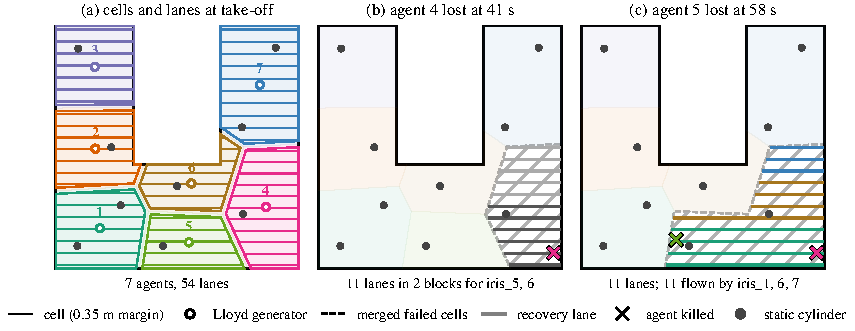
\includegraphics[width=\textwidth]{figures/fig_concept_high.pdf}
\caption{High-level planning in the \Hinf{} U-shape mission, reproduced with the planner code
(centroids within \ConceptCentroidErr~cm of the log, identical lane counts). (a) Cells after the
0.35~m margin with \ConceptRowsTotal{} lanes; each cell's first and last lane follow its boundary.
(b) Agent \ConceptDeadA{} is lost; its cell is re-planned into \ConceptRecRowsA{} lanes in blocks
for agents \ConceptHelpersA. (c) Helper \ConceptDeadB{} is lost too; both cells are merged into
\ConceptRecRowsB{} lanes for agents \ConceptHelpersB, coloured by the agent that flew them
(from telemetry). Lanes ignore obstacles by design.}
\label{fig:concept_high}
\end{figure*}

\headingtwo{Mid Level: Obstacle Mapping and CBF-QP Safety Filter}
\emph{Obstacle map.} Each 360-ray scan is cleaned of returns within 0.55~m of other agents and 0.80~m of the arena
boundary, clustered, and each cluster is fitted with a circle. Detections are associated into one
swarm-wide track list; a track is confirmed after 12 hits and rejected if it moves. Static
obstacle rows use only confirmed tracks, so the swarm starts with an empty map, and the planner
deliberately ignores obstacles, leaving avoidance entirely to the safety filter. The two moving
obstacles are supplied from simulator odometry, i.e.\ they are assumed to be tracked perfectly.

\emph{Actuator-consistent barrier.} With the reference rule $\mathbf{p}_{\mathrm{ref}}=\mathbf{p}+T_{\mathrm{lead}}\mathbf{u}$, the
outer PID makes the commanded-velocity response first order with an acceleration limit,
$\dot v=\mathrm{sat}_{\pm a_{\max}}\bigl(k_v(u-v)\bigr)$, where
\begin{equation}
    k_v=gK_d,\qquad a_{\max}=g\tan\theta_{\max},\qquad
    T_{\mathrm{lead}}=\frac{K_d-k_{\mathrm{ff}}}{K_p},\qquad v_c=\frac{a_{\max}}{k_v},
    \label{eq:plant}
\end{equation}
with $\theta_{\max}=15^\circ$ and $k_{\mathrm{ff}}=0.15$~rad\,s/m. With the LQR outer-loop gains
(used for both controllers) $k_v=\PlantKv$~s$^{-1}$, $a_{\max}=\PlantAmax$~m/s$^2$,
$T_{\mathrm{lead}}=\PlantTlead$~s and $v_c=\PlantVc$~m/s. The stopping distance from speed
$s>v_c$ is $D(s)=(s^2+v_c^2)/2a$; requiring that the distance travelled during a lumped dead time
$T_d=0.40$~s plus $D(s)$ fit inside the clearance $h$ gives the admissible approach speed
\begin{equation}
    \varphi(h)=
    \begin{cases}
        \max\Bigl(0,\,-aT_d+\sqrt{\max\bigl(0,\,a^2T_d^2+2ah-v_c^2\bigr)}\Bigr), & h\ge 0,\\
        \gamma_r\,h, & h<0,
    \end{cases}
    \label{eq:phi}
\end{equation}
which is exactly zero for $h\le v_c^2/2a$, unlike a linear $\gamma h$
(Fig.~\ref{fig:concept_cbf}a); the branch $h<0$ ($\gamma_r=3.5$~s$^{-1}$) demands an outward
velocity once the set has been left. The budget is
$a=\max\bigl(0.15a_{\max},\,\mu a_{\max}-|a_{\mathrm{obs}}|-|a_{\mathrm{wind}}|\bigr)$ with
$\mu=0.75$ (0.85 for walls) and a wind allowance of 0.5~m/s$^2$.

\emph{Quadratic program.} For an obstacle or neighbour at $\mathbf{o}$ with
$\hat{\mathbf{n}}=(\mathbf{p}-\mathbf{o})/\|\mathbf{p}-\mathbf{o}\|$, the condition
$\dot h\ge-\varphi(h)$ is the linear row
\begin{equation}
    -\hat{\mathbf{n}}^{\top}\mathbf{u}\le\lambda\,\varphi(h)-\hat{\mathbf{n}}^{\top}\mathbf{v}_{o},
    \qquad h=\|\mathbf{p}-\mathbf{o}\|-(\rho+r_d+\delta),
    \label{eq:row}
\end{equation}
with drone radius $r_d=0.22$~m, obstacle radius $\rho$ (fitted radius $+0.05$~m for mapped
cylinders, 0.50~m for moving ones), margins $\delta=0.35$~m (static) and 0.75~m (moving), and
$\lambda=1$ for obstacles. Neighbour rows are reciprocal ($\lambda_{ij}+\lambda_{ji}=1$, weighted
by mission state) at a hard radius of 0.70~m and a soft radius of 1.20~m; walls and the end of
the current lane give half-plane rows, and inscribed polygons bound the speed (3~m/s) and the
per-tick change of $\mathbf{u}$. Each agent then solves
\begin{equation}
    \mathbf{u}^\star=\arg\min_{\mathbf{u}\in\mathbb{R}^2}\bigl\|\mathbf{u}-\mathbf{z}\bigr\|^2
    \ \ \text{s.t.}\ \ A\mathbf{u}\le\mathbf{b},\qquad
    \mathbf{z}=\frac{\mathbf{u}_{\mathrm{des}}+\mathbf{t}+w\,\mathbf{u}_{\mathrm{prev}}}{1+w},
    \label{eq:qp}
\end{equation}
exactly, by enumerating the unconstrained point, the projections onto every row and the pairwise
vertices (Fig.~\ref{fig:concept_cbf}b). A tangential bias $\mathbf{t}$, applied within a
60$^\circ$ cone of a head-on approach, breaks symmetric deadlocks and enters only the objective;
$w=0.25$ smooths successive commands. If the QP is infeasible, soft rows are released (tier~1),
then the violation of the hard rows is minimised (tier~2), and a scaled previous command is the
last resort (tier~3).

\begin{figure*}[!tb]
\centering
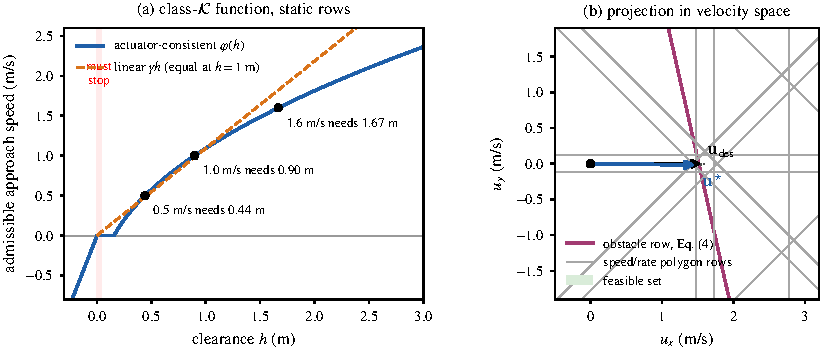
\includegraphics[width=\textwidth]{figures/fig_concept_cbf.pdf}
\caption{Mid-level safety filter with the mission parameters. (a) $\varphi(h)$ of
Eq.~\eqref{eq:phi} for static rows: zero below $h=\CbfHzero$~m, and $h\ge\CbfHsweep$~m is needed
to approach at 1.6~m/s; a linear $\gamma h$ equal at 1.6~m/s permits approach where $\varphi$
demands a stop. (b) One QP solve by the flight code, illustrative case (east sweep at 1.6~m/s,
mapped cylinder \CbfExDist~m ahead, $h=\CbfExH$~m): the row of Eq.~\eqref{eq:row} cuts the
rate-limited set, and the closing speed drops from \CbfExCloseDes{} to \CbfExCloseStar~m/s.}
\label{fig:concept_cbf}
\end{figure*}

\headingtwo{Low Level: LQR and $H_\infty$ Gain Synthesis}
Each axis is modelled about hover as a double integrator $\dot{\mathbf{x}}=A\mathbf{x}+Bu$
(e.g.\ $B=[0,\ g]^\top$ from pitch to $x$, $B=[0,\ 1/I_y]^\top$ from torque to pitch) and
augmented with an integrator on the input, $\mathbf{x}_a=[\mathbf{x}^\top,u]^\top$. The LQR
design solves the algebraic Riccati equation (ARE) for $K_a=R^{-1}B_a^\top P$. The $H_\infty$
design treats a disturbance entering through the input channel, $B_w=[B^\top,0]^\top$, and
solves
\begin{equation}
    A_a^\top P+PA_a+Q_a-P\bigl(B_aR^{-1}B_a^\top-\gamma^{-2}B_wB_w^\top\bigr)P=0,
    \label{eq:hare}
\end{equation}
rejecting solutions for which $A_a-B_aK_a$ is not Hurwitz \cite{doyleStateSpaceHinf1989}, with
$\gamma=1.3\,\gamma_{\min}$ and $\gamma_{\min}$ found by bisection. The state-feedback gain is
mapped to PID form through the pseudo-inverse of
$\Gamma=[C^\top,(CA)^\top,(CA^2)^\top;\,0,(CB)^\top,(CAB)^\top]$; the synthesised inner integral
gain is not used. Figure~\ref{fig:tick} shows where the gains enter the signal path of one control
step, and Table~\ref{tab:gains} lists weights, attenuation levels and gains.

\begin{figure*}[!tb]
\centering
\begin{tikzpicture}[x=1cm,y=1cm,font=\scriptsize,>={Latex[scale=0.7]},
    blk/.style={draw=black!70, rounded corners=1.5pt, fill=white, align=center, inner sep=1.5pt,
                minimum height=1.12cm},
    lbl/.style={font=\scriptsize, align=center, text=black!80},
    row/.style={font=\scriptsize\itshape, text=black!65}]
  \fill[magenta!6, rounded corners=3pt] (-0.1,2.3) rectangle (13.85,4.05);
  \fill[orange!9,  rounded corners=3pt] (-0.1,-0.45) rectangle (13.85,1.85);
  \node[row, anchor=north west] at (-0.05,4.02) {coordinator: every 50 ms, per agent};
  \node[row, anchor=north east] at (13.8,1.82) {flight controller: every 4 ms (each odometry message)};
  % ---- coordinator ----
  \node[blk, text width=3.45cm] (b1) at (1.75,3.0)
    {\textbf{(1) lane follower}\\ $\mathbf{u}_{\mathrm{des}}=v_s\hat{\mathbf{e}}-\mathrm{sat}(k\,e_\perp)\,\hat{\mathbf{n}}$\\ ramped to zero at the lane end};
  \node[blk, text width=3.75cm] (b2) at (5.85,3.0)
    {\textbf{(2) CBF-QP}, Eq.~\eqref{eq:qp}\\ rows: mapped obstacles, moving\\ obstacles, neighbours, walls $\to\mathbf{u}^\star$};
  \node[blk, text width=5.5cm] (b3) at (10.9,3.0)
    {\textbf{(3) set-point}\\ $\mathbf{p}_{\mathrm{ref}}=\mathbf{p}+T_{\mathrm{lead}}\mathbf{u}^\star$, clamped to the lane end\\ and pushed out of the keep-out discs};
  % ---- flight controller ----
  \node[blk, text width=2.75cm] (b4) at (1.4,0.9)
    {\textbf{(4) pre-filter}\\ second order, $\omega_n=8$~rad/s,\\ $\zeta=0.95$, $|\dot{\tilde p}|\le1.8$~m/s};
  \node[blk, text width=4.05cm] (b5) at (5.2,0.9)
    {\textbf{(5) outer PID}, body frame\\ $\theta_{\mathrm{ref}}=K_pe_x+K_i\!\int\!e_x-K_dv_x+k_{\mathrm{ff}}u^\star_x$\\ $|\theta_{\mathrm{ref}}|\le15^\circ$, slew $\le240^\circ$/s};
  \node[blk, text width=3.3cm] (b6) at (9.25,0.9)
    {\textbf{(6) inner PD}\\ $\tau_y=K^{\mathrm{in}}_p(\theta_{\mathrm{ref}}-\theta)-K^{\mathrm{in}}_d\,q$\\ $|\tau|\le0.8$~N\,m, level-out $>25^\circ$};
  \node[blk, text width=2.45cm] (b7) at (12.45,0.9)
    {\textbf{(7) mixer}\\ roll/pitch priority,\\ $\Omega_i^2\in[250^2,1050^2]$};
  \node[blk, fill=teal!9, text width=2.0cm, minimum height=3.6cm] (gz) at (15.2,1.8)
    {\textbf{Gazebo}\\[2pt] 6-DOF body,\\ rotor thrust\\[4pt] odometry 250~Hz\\ LiDAR 10~Hz};
  % ---- signals ----
  \draw[->] (b1) -- (b2);
  \draw[->] (b2) -- (b3);
  \draw[->] (b3.south) -- (10.9,2.08) -- (1.4,2.08) -- (b4.north);
  \node[lbl, fill=white, inner sep=1pt] at (8.0,2.08) {target pose $\mathbf{p}_{\mathrm{ref}}$ and feed-forward $\mathbf{u}^\star$ (ROS~2 topics)};
  \draw[->] (5.2,2.08) -- (b5.north);
  \draw[->] (b4) -- (b5);
  \draw[->] (b5) -- (b6);
  \draw[->] (b6) -- (b7);
  \draw[->] (b7.east) -- node[above, lbl]{$\Omega$} (gz.west |- b7.east);
  \draw[->] (gz.north) -- ++(0,0.3) -| node[pos=0.25, above, lbl]{LiDAR scans $\to$ obstacle map} (b2.north);
  \draw[->, black!55] (15.95,4.45) node[above, lbl, black!70]{wind $\mathbf{w}$} -- (15.95,3.62);
  \draw[decorate, decoration={brace, amplitude=3pt, mirror}, black!60] (3.2,0.26) -- (10.85,0.26)
    node[midway, below=2pt, lbl]{gains from the ARE (\LQR) or the HARE (\Hinf), Table~\ref{tab:gains}};
\end{tikzpicture}
\caption{Signal path of one control step. The coordinator (1)--(3) publishes a set-point and a
velocity feed-forward every 50~ms; the flight controller (4)--(7) runs on each 4~ms odometry
message. The controllers differ only in the gains of (5)--(6) and in the position integrator
(\Hinf: always active, clipped to $\pm0.6$; \LQR: active within 0.25~m, clipped to $\pm0.4$).}
\label{fig:tick}
\end{figure*}

% =====================================================================
\headingtwo{Simulation Setup}
% =====================================================================
Seven 3DR Iris quadrotors ($m=1.50$~kg, $I_{xx}=I_{yy}=0.0291$, $I_{zz}=0.0552$~kg\,m$^2$, arm
0.22~m, $k_f=8.549\times10^{-6}$~N\,s$^2$, rotor speed $\le1100$~rad/s) are simulated in Gazebo
\cite{koenigGazebo2004} with ROS~2. Controllers read ground-truth odometry; no state estimator
is in the loop. Missions start from a launch pad south of the region, cruise at 2.0~m and sweep
at 1.6~m/s. Four regions inside a $28\times28$~m box are used (Fig.~\ref{fig:traj}): \emph{rect}
(784~m$^2$), \emph{L-shape} (588~m$^2$), \emph{U-shape} (624~m$^2$, 10~m wide notch) and
\emph{plus} (460~m$^2$, 10~m wide arms), each with nine vertical cylinders ($r=0.40$~m, 4~m
tall) placed inside the region. All missions use the same combined-hazard scheme:
\begin{itemize}[leftmargin=1.2em,itemsep=0pt,topsep=1pt,parsep=0pt]
\item \emph{Wind.} A first-order Gauss--Markov process per horizontal axis ($\sigma=2.5$~m/s,
      correlation time 0.5~s, seed 42), a surrogate for the Dryden and von K\'arm\'an
      models used in quadrotor studies \cite{mirandaMoyaTurbulentWind2023}, plus a constant $-2$~m/s mean on both
      axes from $t=5$~s, uniform in space and applied through the Gazebo wind-effects plugin
      (vertical component scaled by 0.4). Recorded mean $(\WindMeanX,\WindMeanY)$~m/s, standard
      deviation $(\WindStdX,\WindStdY)$~m/s, horizontal peaks \WindMaxH~m/s.
\item \emph{Moving obstacles.} Two kinematic cylinders ($r=0.45$~m) oscillate along the region
      diagonals with amplitude 10~m (12~m, offset by 1~m, in \emph{plus}) at 0.15 and 0.11~rad/s,
      i.e.\ peak speeds of 1.6--2.6~m/s.
\item \emph{Agent loss.} When coverage first reaches 18\% and 32\%, one pre-selected agent is
      killed (rotor speeds set to zero, fail-stop) and the coordinator is notified at once.
      Victims were chosen to own comparable cells next to the launch pad (Table~\ref{tab:results}).
\end{itemize}
Both controllers use the same planner, filter and plant model; Eq.~\eqref{eq:plant} is evaluated
with the LQR outer-loop gains in both cases. Each region--controller pair was flown once
($N=1$) and recorded on video. The two \emph{plus} missions also include three transit guards
added before they were flown (a stall detector, a speed reduction above 16$^\circ$ tilt and a
20~s start-wait timeout). Metrics are computed from 20~Hz controller logs, discarding the rows
after an agent is killed and the first 20~s. Lateral error is the deviation from the lane
reference during steady east--west sweeps (heading stable for 1.5~s, speed above 0.6~m/s);
torque effort is the time average of $\tau_x^2+\tau_y^2$; obstacle distance is measured from the
drone centre to the cylinder surface. The collision geometry of the airframe reaches
\BodyHalf~m (body) to \RotorReach~m (rotor tips) from its centre, so a surface distance below
these values means certain or possible contact.

\begin{table}[!tb]
\centering
\caption{Gain synthesis (outer $x$/$y$ and inner roll/pitch loops) and linear analysis of the
outer loop with the inner loop closed. $\|G\|_\infty$: peak gain from a disturbance acceleration
to position; PM/GM: phase and gain margins of the outer loop.}
\label{tab:gains}
\footnotesize
\setlength{\tabcolsep}{4pt}
\begin{tabular}{@{}l l l c c c c c c c@{}}
\toprule
Design & Loop & $Q$, $R$ & $\gamma_{\min}\!\to\!\gamma$ & $K_p$ & $K_i$ & $K_d$ & $\|G\|_\infty$ (s$^2$) & PM & GM \\
\midrule
\multirow{2}{*}{\LQR} & outer & diag(0.08, 0.35), 1 & -- & \KoutkpLqr & \KoutkiLqr & \KoutkdLqr & \multirow{2}{*}{\HnormLqr} & \multirow{2}{*}{\PmLqr$^\circ$} & \multirow{2}{*}{\GmLqr~dB} \\
 & inner & diag(6, 0.6), 0.05 & -- & \KinkpLqr & -- & \KinkdLqr & & & \\
\multirow{2}{*}{\Hinf} & outer & diag(0.10, 0.40), 1 & 2.54$\to$3.30 & \KoutkpHinf & \KoutkiHinf & \KoutkdHinf & \multirow{2}{*}{\HnormHinf} & \multirow{2}{*}{\PmHinf$^\circ$} & \multirow{2}{*}{\GmHinf~dB} \\
 & inner & diag(4, 0.4), 0.06 & 2.54$\to$3.31 & \KinkpHinf & -- & \KinkdHinf & & & \\
\bottomrule
\end{tabular}
\end{table}

\begin{table*}[!tb]
\centering
\caption{Mission results. $T$: mission time; lat.: RMS lateral sweep error; $\bar v$: mean sweep
speed; alt.: RMS altitude error; tilt: 95th percentile while sweeping, and maximum; effort: mean
$\tau_x^2+\tau_y^2$ (N$^2$m$^2$); $d_{\mathrm{obs}}$, $d_{\mathrm{v2v}}$: minimum centre-to-surface
distance to a static cylinder and minimum inter-agent distance; tier: QP solves needing tier 1
or 2. Killed agents: rect \VictimsRectHinf{} (H$_\infty$), \VictimsRectLqr{} (LQR); L-shape
\VictimsLshapeHinf; U-shape \VictimsUshapeHinf; plus \VictimsPlusHinf. \LQR{} rect covers the
\TmisRectLqr~s before its abort.}
\label{tab:results}
\footnotesize
\setlength{\tabcolsep}{3.2pt}
\begin{tabular}{@{}l l c c c c c c c c c c c c@{}}
\toprule
Region & Controller & Status & Cov. (\%) & $T$ (s) & lat. (cm) & $\bar v$ (m/s) & alt. (cm)
 & tilt$_{95}$ ($^\circ$) & tilt$_{\max}$ ($^\circ$) & effort & $d_{\mathrm{obs}}$ (m) & $d_{\mathrm{v2v}}$ (m) & tier (\%) \\
\midrule
\csname @@input\endcsname generated/table_results.tex
\bottomrule
\end{tabular}
\end{table*}

\begin{figure*}[!tb]
\centering
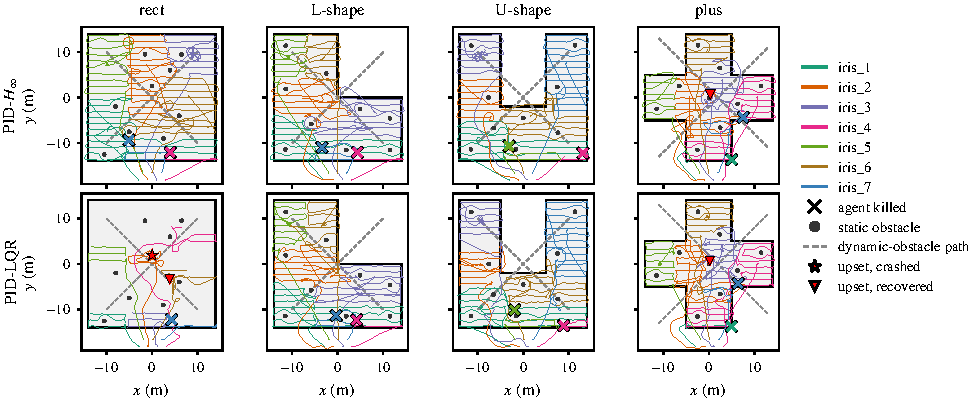
\includegraphics[width=\textwidth]{figures/fig_traj.pdf}
\caption{Flown trajectories of live agents above 0.5~m, including transit from the launch pad
($y\approx-18$~m). Dark discs: static cylinders; dashed: moving-cylinder paths; crosses: agent
kills; red markers: tilt upsets above 30$^\circ$.}
\label{fig:traj}
\end{figure*}

% =====================================================================
\headingone{Results and Discussion}
% =====================================================================

\headingtwo{Mission Completion and Fault Recovery}
Table~\ref{tab:results} and Fig.~\ref{fig:traj} summarise the eight missions. Seven finished
with every surviving agent back at its cell centroid and final coverage of \CovMin--\CovMax\%,
although two of seven agents (28.6\%) were lost at 18\% and 32\% coverage. In every mission the
obstacle map contained all nine cylinders (centre and radius within the 0.1~m log resolution)
plus at most two unmatched tracks, and no completed mission needed a tier-3 fallback. After each
kill the coverage curve drops slightly, because the coverage of the failed cell is erased, and
then resumes its slope (Fig.~\ref{fig:coverage}); Fig.~\ref{fig:env} shows the final maps. The
\LQR{} U-shape mission ended just below the 97\% target (\CovUshapeLqr\%) with thin uncovered
strips along cell boundaries in the left arm that are nearly absent in the \Hinf{} map; we did
not isolate their cause. The \LQR{} rect mission was aborted at \TmisRectLqr~s (see below).

\begin{figure*}[!tb]
\centering
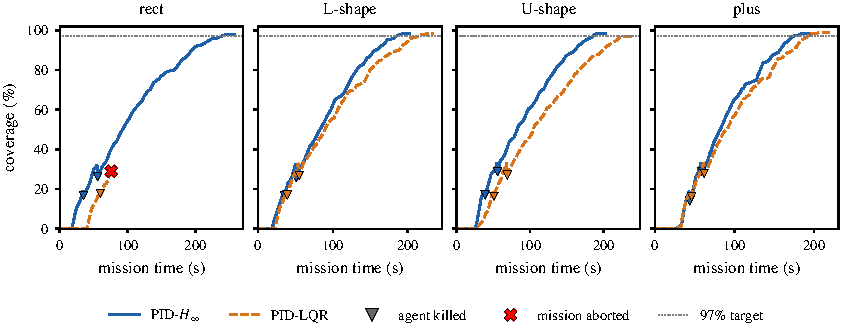
\includegraphics[width=\textwidth]{figures/fig_coverage.pdf}
\caption{Coverage against mission time (coordinator clock, 1~Hz). Triangles mark agent kills;
the step after each kill is the erased coverage of the failed cell being re-swept.}
\label{fig:coverage}
\end{figure*}

\begin{figure}[!tb]
\centering
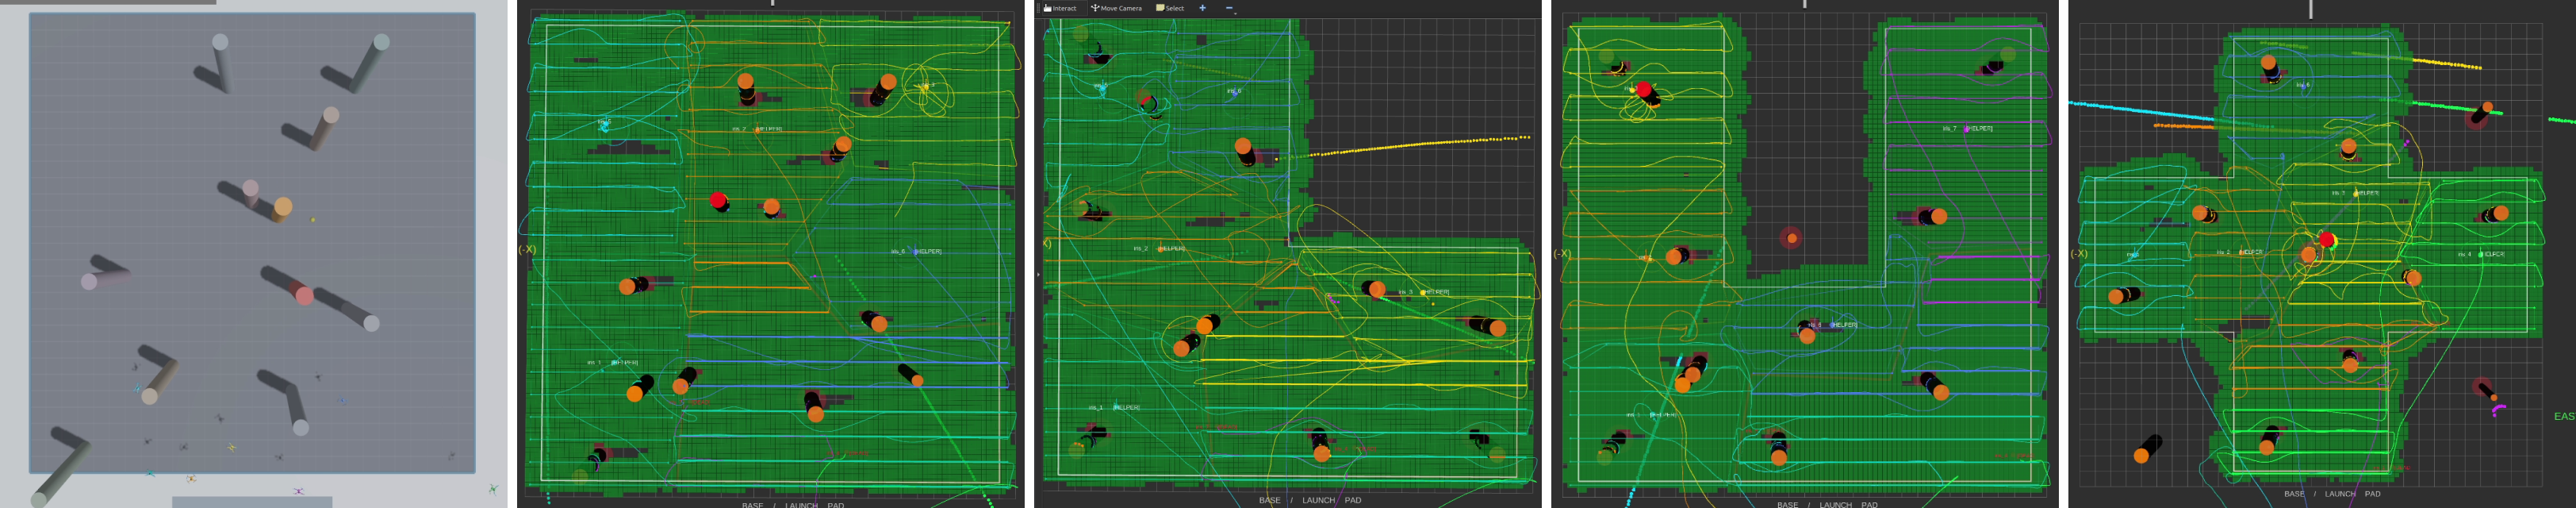
\includegraphics[width=\textwidth]{figures/fig_env.png}
\caption{(a) Gazebo view of the rect mission; (b)--(e) RViz coverage maps (green) at the end of
the \Hinf{} missions in rect, L-shape, U-shape and plus, with lanes, flown paths and mapped
obstacles. Frames are extracted from the mission recordings.}
\label{fig:env}
\end{figure}

\headingtwo{Tracking under Turbulence: LQR versus $H_\infty$ Gains}
The two designs differ clearly in how tightly they hold a lane (Fig.~\ref{fig:tracking}a): the
median lateral error was \LatMedHinfMin--\LatMedHinfMax~cm with \Hinf{} and
\LatMedLqrMin--\LatMedLqrMax~cm with \LQR{}, and the RMS error fell from
\LatRmsLqrMin--\LatRmsLqrMax~cm to \LatRmsHinfMin--\LatRmsHinfMax~cm, a
\LatRedMin--\LatRedMax\% reduction in all four regions. Most of the difference is a mean offset:
\LQR{} flew $\LatMeanLqrMax$ to $\LatMeanLqrMin$~cm downwind (the mean wind blows towards $-y$),
\Hinf{} within \LatMeanHinfMin--\LatMeanHinfMax~cm of the lane, while the standard deviations
differed less (\LatStdHinfMin--\LatStdHinfMax{} vs \LatStdLqrMin--\LatStdLqrMax~cm). This is a
low-frequency effect: the $H_\infty$ outer integral gain is \KiRatio{} times larger, and the
\LQR{} node freezes its position integrator when the error exceeds 0.25~m, which happened in
\IntegOffLqrMin--\IntegOffLqrMax\% of its sweep samples. The mean sweep speed was
\VHinfMin--\VHinfMax~m/s against \VLqrMin--\VLqrMax~m/s for a 1.6~m/s command, which accounts
for the \TimeRedMin--\TimeRedMax\% shorter missions; altitude error and 95th-percentile tilt were
essentially equal. The linear analysis (Table~\ref{tab:gains}) agrees in direction: the $H_\infty$
gains lower the worst-case gain from disturbance acceleration to position by a factor of
\HnormRatio{} and the position deviation under the Gauss--Markov input by \SigxRatio{}
(Fig.~\ref{fig:tracking}c).

The price is a higher effort: \Hinf{} used \EffRatioMin--\EffRatioMax{} times the torque effort
of \LQR{} in the completed pairs (Fig.~\ref{fig:tracking}b), with motor saturation below 0.2\% of
samples in every mission, and a higher outer-loop crossover (\WcHinf{} vs \WcLqr~rad/s) with
smaller margins. The measured reduction is far smaller than the linear factor because the tilt
limit, the reference pre-filter, the QP rate limits and the wind force model are absent from the
linear model. As the weights $Q$, $R$ differ and the integrator gating belongs to the \LQR{} node
rather than to the synthesis, the comparison is between two complete gain designs; the
contribution of $\gamma$ is not isolated from that of higher loop gain.

\begin{figure*}[!tb]
\centering
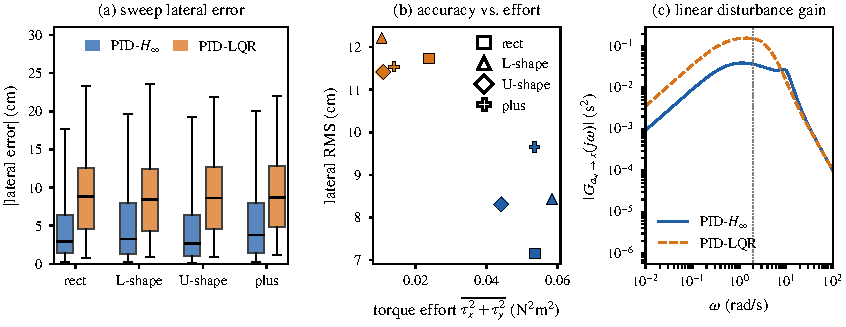
\includegraphics[width=\textwidth]{figures/fig_tracking.pdf}
\caption{(a) Absolute lateral error during steady east--west sweeps (box: quartiles, whiskers:
5th--95th percentiles). (b) RMS lateral error against torque effort per mission. (c) Gain from a
disturbance acceleration to position of the linearised outer loop; dotted: corner frequency of
the wind model.}
\label{fig:tracking}
\end{figure*}

\headingtwo{Safety: Clearance, Contact and Upset Events}
No two agents came closer than \VtwovLshapeLqr~m (\LQR{}, L-shape), above the 0.70~m hard
radius. The minimum surface distance to static cylinders under \Hinf{} was \ObssurfRectHinf,
\ObssurfLshapeHinf{} and \ObssurfUshapeHinf~m in rect, L- and U-shape, clear of the airframe,
and under \LQR{} \ObssurfRectLqr, \ObssurfLshapeLqr{} and \ObssurfUshapeLqr~m; in \emph{plus}
both controllers passed within \ObssurfPlusHinf~m of the central cylinder, inside the rotor
envelope. The resulting upsets (Fig.~\ref{fig:events}) share a pattern in the coordinator log:
each happened while the agent stepped to its next lane beside a cylinder, after the QP had run in
tier~2 for \TierSpanMin--\TierSpanMax~s with that cylinder as the binding row. In the \LQR{} rect
mission agent 2 came within \UpRectLqrSurf~m of the cylinder at $(0,2.5)$, i.e.\ body contact,
tilted to \UpRectLqrTilt$^\circ$ and fell. In \emph{plus}, agent 2 of both missions grazed the
central cylinder: under \LQR{} the tilt reached \UpPlusLqrTilt$^\circ$ with little height loss,
under \Hinf{} \UpPlusHinfTilt$^\circ$ with a drop to \UpPlusHinfZmin~m before cruise altitude was
regained within about 3~s. With one run per case these events cannot be attributed to the
controller; they are better explained by obstacle-blind lanes whose ends and steps fall inside
the margin of a cylinder, combined with a barrier built on a 0.22~m disc and a fixed
0.5~m/s$^2$ wind allowance that gusts of up to \WindMaxH~m/s exceed. A further
\UpRectLqrSecondTilt$^\circ$ upset (\LQR{}, rect, agent 6 at \UpRectLqrSecondT~s) occurred in
transit away from any cylinder and was recovered. Moving obstacles also entered their 0.75~m
margin: tier-2 logs show negative barrier values in \NRunsHdynNeg{} of eight missions, the lowest
($\HdynMinLogged$~m) corresponding to a surface distance of \DynSurfMinLogged~m; being logged
only in tier~2, these values bound the true minimum from above. A rotor-tip collision envelope,
obstacle-aware lane ends and a gust-dependent acceleration budget are the obvious remedies.

\begin{figure}[!tb]
\centering
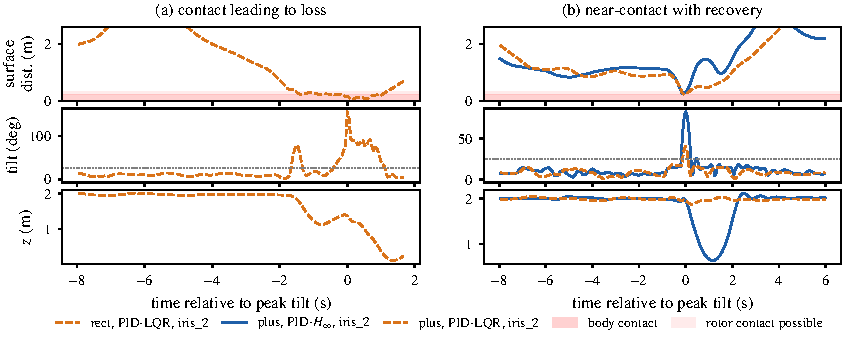
\includegraphics[width=\textwidth]{figures/fig_events.pdf}
\caption{Upset events, aligned at peak tilt. Top: centre-to-surface distance to the nearest
static cylinder (dark band: body contact, light band: rotor contact possible); middle: tilt
(dotted: 25$^\circ$ level-out threshold); bottom: altitude. (a) \LQR{}, rect, agent 2: contact
and loss. (b) \emph{plus}, agent 2 under both controllers: grazing contact and recovery.}
\label{fig:events}
\end{figure}

\headingtwo{Limitations}
The results rest on one run per configuration with a fixed wind seed, perfect state feedback,
perfectly tracked moving obstacles, instantaneous failure detection, a geometric coverage model
without camera error, and centralised execution of the upper layers; no component was ablated or
compared with a re-implemented baseline.

% =====================================================================
\headingone{Conclusion}
% =====================================================================
A three-layer architecture combining polygon-clipped Voronoi partitioning, boundary-following
sweeps, lane-level fault reallocation, a LiDAR-mapped actuator-consistent CBF-QP and
Riccati-synthesised PID control was evaluated in eight simulated missions with seven quadrotors
under strong turbulence, unmapped and moving obstacles, and the loss of two agents. Seven
missions finished with \CovMin--\CovMax\% coverage. Gains from the $H_\infty$ Riccati equation
held the lanes \LatRedMin--\LatRedMax\% more tightly and shortened missions by
\TimeRedMin--\TimeRedMax\% compared with LQR gains, at several times the torque effort and with
smaller margins; both designs suffered obstacle contacts in gusts, one of which ended an LQR
mission. Future work will repeat the campaign over many wind seeds, enlarge the collision envelope
and add wind to the barrier model, distribute the upper layers onto the vehicles, and move to
flight tests with on-board state estimation.

\ifanon\else
\headingone{Acknowledgments}
The authors thank the Center for Instrumentation Technology and Automation, Institut Teknologi
Bandung, for supporting this work.
\fi

\headingone{References}
{\small
\renewcommand{\section}[2]{}
\bibliographystyle{aipnum4-1-epic}
\bibliography{references}
}

\end{document}
